\documentclass[twocolumn,10pt,dvipdfmx,a4paper]{jsarticle}

\usepackage[margin=15mm]{geometry} %余白の削除

\usepackage{amsmath,amssymb}
\usepackage{bm}
\usepackage[dvipdfmx]{graphicx}
\usepackage{physics} % http://mirrors.ibiblio.org/CTAN/macros/latex/contrib/physics/physics.pdf
\usepackage{siunitx} %SI単位を楽に出力
\usepackage{mathtools} %環境の追加
% \usepackage{circuitikz} %電気回路をtex中で書く
% \usepackage{caption} %番号なしキャプションを書く
% \usepackage{cancel} %式中に斜線を入れる
% \usepackage{tensor} %テンソルの添え字を書く
% \usepackage{tikz} %図を書く
% \usepackage{ascmac} %四角い枠の中に文章を書く
% \usepackage{float} %figureで[hbp]オプションを使う
% \usepackage{hyperref}  \usepackage{pxjahyper} %ハイパーリンクをつかう
% \usepackage{tablefootnote} %表中に注釈をいれる
% \usepackage[thicklines]{cancel} %数式中の取り消し線
% \usepackage[version=4]{mhchem} %化学式の入力
\usepackage{pdfpages}
% \usepackage{wrapfig} %文章の回り込み
\usepackage[subrefformat=parens]{subcaption} %(a)図のようにすることができるやつ
\usepackage{here}
\usepackage{url}
\usepackage{mathrsfs}

\graphicspath{{./image/}}

\renewcommand{\abstractname}{Abstract}

\title{量子多体系とニューラルネットワーク}
\author{1522068 西原翔}
\date{\today}

\begin{document}
\twocolumn[
\maketitle

\begin{abstract}
    The application of neural networks in condensed matter physics
    is transforming the field by handling complex and large datasets.
    Neural networks facilitate rapid material discovery
    by predicting physical properties like thermal and electrical conductivity from vast datasets,
    significantly speeding up the process compared to traditional methods.

    In this report, I'm going to introduce the representation of wave functions
    using neural networks and apply 1D AntiFeromagnetic Heisenberg model
    to obtain ground state of the system and the correlation of each spins.
    The parameters of the neural networks is optimized
    by Stochastic Reconfiguration method (SR method).
\end{abstract}]
\section{始めに}
SGC ライブラリ「量子多体系とニューラルネットワーク」\cite{SGC191}
のなかで、ボルツマンマシンを用いた量子多体系の紹介があった。
ただ、このテキストでは大まかな紹介になっていて、
具体的な話は元の Carleoらの元の論文など\cite{Carleo-2017}\cite{Carleo-2018}を見るようにというようにあった。
そこで、このレポートはCarleo の元の論文\cite{Carleo-2017}を追っていくつもりである。

\section{量子多体系の扱われ方}
実際にニューラルネットワークがどのように量子多体系に応用されているかを見る前に、
そのモチベーションを見ていこう。

量子力学において系の状態はハミルトニアンと呼ばれる演算子の固有値方程式で表される。
固有ベクトルは波動関数と呼ばれ、固有値は系のエネルギーとなる。
量子一体問題の例として、
電子がクーロン引力によって陽子に束縛される水素原子原子を考える。
\footnote{実はこれは二体問題であるのだが、
重心運動と相対運動に分離することができ、相対運動にだけ注目すると一体問題になる。}
この系の状態は次のシュレディンガー方程式と呼ばれる固有値方程式で書かれる。
\begin{equation}
    \qty(-\frac{1}{2}\laplacian -\frac{1}{r})\psi(\vb*{r})=E\psi(\vb*{r})
\end{equation}
\footnote{ここでは原子単位系と呼ばれる単位系を用いて無次元化している。}
この時点で複雑な偏微分方程式になっていることがわかる。

では\(N_e\)個の電子が結晶中に固定された\(N_n\)個原子核からのクーロンポテンシャルを受けながら、
電子同士もクーロン相互作用をするような状態の固有値方程式は次のようになる。
\begin{align}
    \sum_{i=1}^{N_n}\sum_{j=1}^{N_e}\qty(-\frac{1}{2}\laplacian_j
    -\frac{1}{\abs{\vb*{R}_i-\vb*{r}_j}}
    +\sum_{k=1}^{N_e}\frac{1}{\abs{\vb*{r}_j-\vb*{r}_k}})\psi = E\psi
    \label{eq:no2}
\end{align}
というようにとても手計算で扱えたものにはなっていない。
また、計算機を使ったものであっても粒子数のべきのオーダーで計算量が増えていく。
そのため、身近にあるパソコンでは 50 個程度電子の系でしかこの計算をすることができない。
これでは実際の物質中のような電子が\num{6.0e23}個もあるような系は到底理理解できないように見える。

しかし物性物理の理論では物理的な解釈をもとにこの偏微分方程式に近似を加えることでさまざまな現象を説明する。
その近似の例を見てみよう。
電子同士の相互作用を無視して、原子核からのクーロン引力ポテンシャルを周期的でとても弱いものとして扱う。
そして、電子の質量に周期的なポテンシャルを繰り込むことで最終的には
\begin{equation}
    -\frac{1}{2m^*}\laplacian F(\vb*{r}) = E F(r)
\end{equation}
という微分方程式にすることができる。
このような近似をしていくのがバンド理論と呼ばれるものである。
これにより金属のとても多くの性質を説明することができる。

これは驚くべきことである。
つまり元の微分方程式ではこまごまとした余計な情報が多く含まれていて、
系の状態を決定づける重要な特徴量は微分方程式を完全に解かずとも得られることを意味する。
従来の物理学ではこの特徴量を理論体系とそれに基づく勘によって探し出していた。
この多自由における特徴量を求めるといった問題はまさに近年発展している機械学習の得意とする問題である。
なので物性物理に限らず物理学の世界において理論物理、実験物理に加え、
新しく計算物理と呼ばれる新領域も物理学会にて作られるようになった。

\section{量子状態とボルツマンマシン}
スピンやボゾン粒子の数といった\(N\)個の離散的な自由度\(\mathcal{S}=(S_1,\,S_2,\,\dots\, S_N)\)をもった量子系を考える。
関数は定義域から値域への写像だということを思い出すと、
この系の波動関数を\(N\)次元の集合\(\mathcal{S}\)というのをある複素数へと移すものだと考えることはできる。
実際、波動関数の形を求めることで何かを得るということは少なくあるエネルギーを持った粒子がどれほどあるかといった情報しか使わない。
なので関数の形はわからずともこと足りる。
この観点から波動関数は完全なブラックボックスとして扱っても問題ないことがわかる。
入力をブラックボックスに通して出力を得るというのは人工ニューラルネットワークモデルのやることである。
以上より波動関数をニューラルネットワークを用いて表すというアイデアが生まれる。

ニューラルネットワークのモデルというのはさまざまある。
一口に量子多体系といってもそれぞれのモデルがどの問題に適しているかというのはもちろん違う。
ここでは制限ボルツマンマシンというニューラルネットワークモデルを用いる。

ボルツマンマシンのアイデアを示していく。
\(N\)個の離散的な自由度\(\mathcal{S}=(\sigma_1^z,\,\sigma_2,\,\dots\, \sigma_N^z)\)を考える。
\(\mathcal{S}\)の各成分の値にはある関係があり、データ空間のごく一部にしか分布しない。
そのデータは確率分布\(p(\mathcal{S})\)に従って生成されたと考える。
するとどのような状態があり得るかどうかという問題は確率分布\(p(\mathcal{S})\)を求める問題となる。
真の確率分布\(p(\mathcal{S})\)はわからないのであるモデル\(p(\mathcal{S}|w)\)を仮定して
そのパラメータ\(w\)を調整する(学習する)ことで真のモデルに近づけることを考える。

ではこのモデルとしてどのようなものがあり得るか考える。
\(\mathcal{S}\)の各成分の値の関係をネットワークにしてそのエッジの重みで状態を表すことが出来そうである。
この場合各成分の間の関係として疑似相関といったことがあり得る。
なのでネットワークに隠れ層の補助自由度として\(M\)成分の\((h_1,\,h_2,\,\dots,\, h_M)\)を導入して
これを通したネットワークになっていると考える。
そうしたときに確率分布は
\begin{align}
    p(\mathcal{S},\,h\, | w ) &= \frac{1}{Z}e^{-E\qty(\mathcal{S},\,h\, | w )}\\
    E(\mathcal{S},\,h\, | w ) &= -\sum_{i=1}^{N} w_i \sigma_i^z - \sum_{j=1}^{M} {w'}_j h_i - \sum_{ij}w_{ij} \sigma_i^z h_j
\end{align}
というようにできそうである。
ここで\(Z\)は規格化定数、\(E(\mathcal{S},\,h\, | w )\)はエネルギー関数、
\(w_i\)は\(\mathcal{S}\)へのバイアス、\({w'}_j\)は\(h\)へのバイアス、
\(w_ij\)は\(\mathcal{S}\)と\(h\)の結合の強さに相当する。
(模式図:図\ref{fig:01})
\begin{figure}
    \centering
    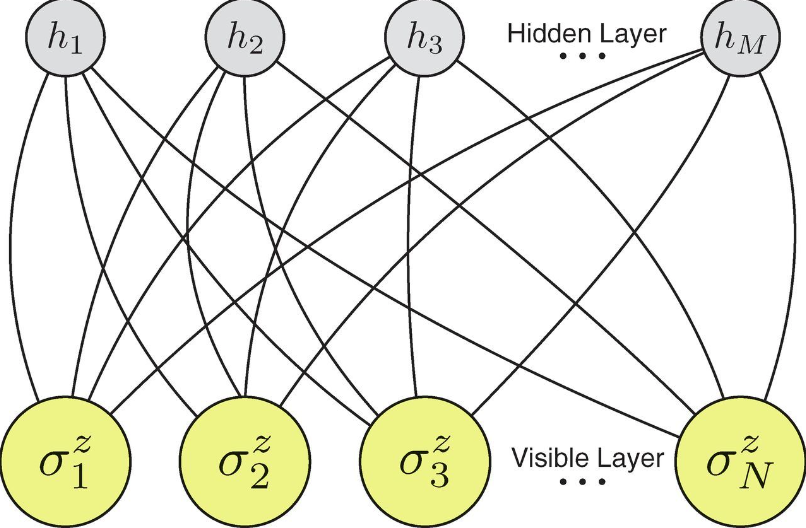
\includegraphics[width=0.9\columnwidth]{01.png}
    \caption{制限ボルツマンマシンの模式図(引用\cite{Carleo-2017})}
    \label{fig:01}
\end{figure}
実際には隠れ相は見えないのでこれの状態についてすべての和を取って周辺確率分布
\begin{equation}
    p(\mathcal{S}|w)=\sum_h \frac{1}{Z}e^{-E\qty(\mathcal{S},\,h\, | w )}
\end{equation}
というのがモデルとなる。
情報を2進数で表示すると自由度が増える代わりに\(\sigma=\pm 1,\,h=\pm1\)とできる。
このようにして和を取ると
\begin{equation}
    p(\mathcal{S}|w)=\exp(\sum_i w_i\sigma_i^z)\times\prod_j 2\cosh({w'}_j+\sum_i w_{ij}\sigma_i^z)
\end{equation}
というようにできる。

何らかのコスト関数を用いてパラメータ\(w\)を変化させていくことで確率分布となる。
量子力学によると確率分布は波動関数の二乗\(p(\mathcal{S})\abs*{\psi(\mathcal{S})}^2\)で表される。
また、実際の系で最も安定な状態はエネルギーが低い状態のことである。
これを量子力学的な表記で表すと
\begin{align}
    E &= \frac{\bra{\psi(\mathcal{S}|w)}\mathcal{H}\ket{\psi(\mathcal{S}|w)}}{\braket{\psi(\mathcal{S}|w)}}\\
    &= \frac{\sum_{\mathcal{S},\, \mathcal{S}'}\psi^*(\mathcal{S}|w)\mathcal{H}(\mathcal{S},\,\mathcal{S}')\psi(\mathcal{S}'|w)}{\sum_\mathcal{S} \abs{\psi(\mathcal{S}|w)}^2}
\end{align}
と表される。なのでこの量を最小化するようにパラメータ\(w\)を学習することとなる。
注意したいのは波動関数自体は複素数なので\(w\)は複素数値になっている。
ここでモデルのパラメータの更新には確率的再配置法(Stochastic Reconfiguration method:SR method)と呼ばれる手法で行われている。
機械学習の分野では、この手法は自然勾配法と呼ばれている方法である。

\section{物理の模型}
今回はスピンという磁石のような量についてのモデルである
反強磁性ハイゼンベルグ模型(AntiFeromagnetic Heisenberg model:AFH)というのを扱う。
直感的には、\(d\)次元の格子点の上に強さが同じ磁石(スピン)を載せたモデルである。
ハイゼンベルグ模型は各磁石の向きは3次元的な方向として扱うモデルで、
反強磁性というのはスピンの向きが互い違い(反平行)である状態が安定するといった意味である。
このモデルを表すハミルトニアン\(\mathcal{H}_{\text{AFH}}\)は
\begin{equation}
    \mathcal{H}_{\text{AFH}} = \sum_{ij} \sigma_i^x\sigma_j^x + \sigma_i^y\sigma_j^y+ \sigma_i^z\sigma_j^z
\end{equation}
として表される。
\(\sigma\)はパウリ行列と呼ばれるもので
\begin{equation}
    \sigma^x = \begin{pmatrix}
        0 & 1\\
        1 & 0
    \end{pmatrix}, \quad
    \sigma^y = \begin{pmatrix}
        0 & -i\\
        i & 0
    \end{pmatrix}, \quad
    \sigma^z = \begin{pmatrix}
        1 & 0\\
        0 & -1
    \end{pmatrix}
\end{equation}
である。

\section{結果}
Fortran で実装したコードは今回参考にしているテキスト\cite{SGC191}を書いた野村先生のウェブページ
(\url{https://sites.google.com/view/yusuke-nomuras-webpage-jp})
にあり、
これを python で書き直したのがこのページ(\url{https://ieyasu03.web.fc2.com/Computer/04_RBM.html})
にあった。
これをもとに自分でも実装し、パソコンに計算をさせてみた。
ただ、ここで実装するうえでは、
系の対称性としてスピンの\(z\)成分の和が一定であることや周期的境界条件とそれに伴う併進対称性というのも考慮する必要があった。
なので条件としては、スピンの数が\(N=8\),
隠れ自由度の数は\(M=N=8\),
スピンの\(z\)成分の和が 0, パラメータの更新回数は 3000 回
というような条件で行った。

すると、基底状態のエネルギーは -14.603878 となった。
厳密解との差は 0.000030 であるのでうまくいっているのがわかる。
系の波動関数は図\ref{fig:02} となった。
横軸の\(x\)はスピンの\(z\)成分を符号化したものであり、別に位置座標ではない。
これを見ると左右対称になっている。
これは系の\(z\)軸の向きをどちらにとってもよいという反転対称性を表している。
なので右半分と左半分ではちょうどスピンの向きが反転した状態になっている。
また、最も高い値が\(x=21, 50\)にある。
これは反強磁性ハイゼンベルグ模型の基底状態であると解釈でき、
その中身は
\begin{equation}
    \psi = (\uparrow,\,\downarrow,\,\uparrow,\,\downarrow,\,\uparrow,\,\downarrow,\,\uparrow,\,\downarrow,\,)
\end{equation}
とこれの上下を反転させたものである。
確かに、ハミルトニアンから予想されるような基底状態担っているのがわかる。
\begin{figure}
    \centering
    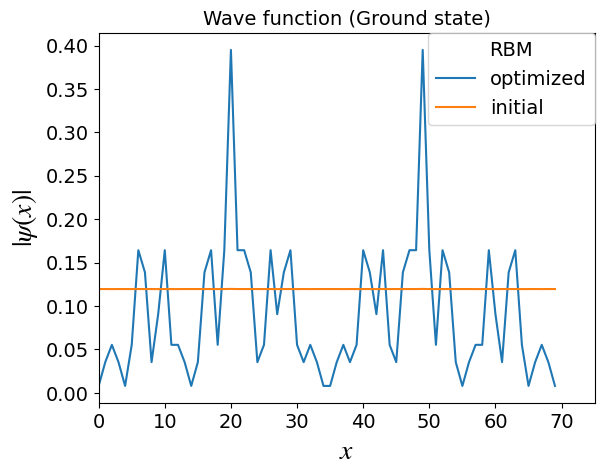
\includegraphics[width=0.9\columnwidth]{02.png}
    \caption{反強磁性ハイゼンベルグ模型の波動関数}
    \label{fig:02}
\end{figure}

ニューラルネットワークの併進対称性を考慮したパラメータ\(w_{i-j}\)は図\ref{fig:03}
のようになった。
これを見ると隣接するスピン同士の影響は大きくて、
遠くにあるほど影響は小さいことがわかる。
\begin{figure}
    \centering
    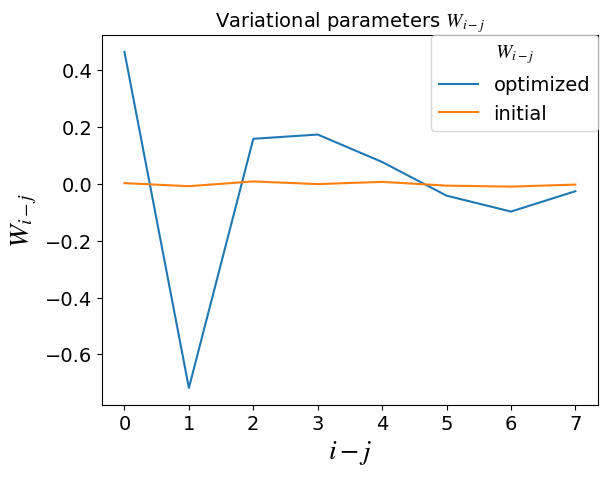
\includegraphics[width=0.9\columnwidth]{03.png}
    \caption{制限ボルツマンマシンのパラメータ\(w_{ij}\)の様子}
    \label{fig:03}
\end{figure}

\section{終わりに}
Carleoの元の論文\cite{Carleo-2017}ではこのレポートで見ていったモデルのほかに
横磁場イジングモデルというのも扱っている。
さらに1次元だけではなく、2次元での計算も行っている。

それらのモデルは量子多体系では最も基本的なモデルのであるが、
これをもとに話を発展させていくことが多い。
この論文により量子多体系においてニューラルネットワークが使えるものであるということがわかったため、
これ以降、機械学習を使った計算による結果が多く出るようになったようである。
機械学習の性質上、
その中のパラメータはブラックボックスになることが多いが、
今回使った制限ボルツマンマシンは統計力学によって解釈をすることができる。
このほかにもニューラルネットワークを場の量子論の枠組みから捕えようとする試みもあるようである。
計算資源が豊富に増えたなか、このリソースを使ってどのような物理ができていくのか楽しみである。

\bibliographystyle{junsrt}
\bibliography{reference}

\end{document}